\documentclass[oneside,12pt,openany]{book}
\usepackage[toc,page]{appendix}
\usepackage{amsmath,amsthm,amsfonts,indentfirst,graphicx,subcaption,textcomp,commath,mathtools,hyperref,pgfplots,epigraph,enumitem,pdfpages}

\hypersetup{
	colorlinks=true,
	linkcolor=blue,
	filecolor=blue,      
	urlcolor=blue,
	citecolor=blue,
	bookmarks=true,
}

\usepackage{scrextend}
\usepackage{afterpage}
\newcommand\blankpage{
	\vfill
	\pagebreak
	\ifthispageodd{\null
		\vfill
		\vfill
		\clearpage}{}
}

\renewcommand{\baselinestretch}{1.5}
\setlength{\textwidth}{6in}

\setlength{\oddsidemargin}{.5in} \setlength{\evensidemargin}{0mm}

\newtheorem{defn}{Definition}[section]
\newtheorem{thm}{Theorem}[section]
\newtheorem{lemma}{Lemma}[section]
\newtheorem{cor}{Corollary}[section]
\newtheorem{prop}{Proposition}[section]
\newtheorem{exa}{Example}[section]
\newtheorem{clm}{Claim}[section]
\newtheorem{rmk}{Remark}[section]
\newtheorem{case}{Case}[section]

\DeclarePairedDelimiter\ceil{\lceil}{\rceil}
\DeclarePairedDelimiter\floor{\lfloor}{\rfloor}
\newcommand{\rpm}{\raisebox{.2ex}{$\scriptstyle\pm$}}

\begin{document}
	\frontmatter
	\begin{titlepage}
		\centering
		{\scshape\Large \textbf{CAPTURING THE PREDICTIVE POWER OF CORTICAL LEARNING ALGORITHMS} \par}
		\vspace{5.5cm}
		{\scshape\large By \par}
		{\scshape\large Alexander C Michels\par}
		\vfill
		{\large Submitted to the Department of Computer Science and Mathematics\par}
		{\large Westminster College, New Wilmington, PA\par}
		{\large In partial fulfillment of the requirements for Honors Research\par}

		\vfill
		advised by\par
		\large
		Carolyn Cuff, Ph.D.\par
		C. David Shaffer, Ph.D.\par
		William Procasky, Ph.D.\par
		
		\vfill
		
		% Bottom of the page
		{\large \today\par}
	\end{titlepage}
	\setcounter{tocdepth}{1}
	\tableofcontents
	\vfill
	\pagebreak
	
	\addcontentsline{toc}{chapter}{Acknowledements}
	\chaptermark{ACKNOWLEDGEMENTS}
	\begin{center}
		\textbf{ACKNOWLEDGEMENTS}
	\end{center}

	\textcolor{red}{Type your acknowledgements here}
	\vfill
	\pagebreak
	
	\addcontentsline{toc}{chapter}{Abstract}
	\chaptermark{ABSTRACT}
	\begin{center}
		\textbf{ABSTRACT}
		
		\begin{quotation}
			\noindent Hierarchical Temporal Memory (HTM) is model of intelligence based on the the interactions of pyramidal neurons in the mammalian neocortex currently being developed by Numenta. It has stood out from other machine learning techniques due to high noise tolerance and learning capacity making it well-suited for anomaly detection, prediction, signal processing, and sensorimotor processes. We seek to find a mathematical analogy to the predictive power of this biologically constrained theory using models from time series analysis. To do this, we statistically analyzed the error in predictions of HTM networks that we asked to predict outputs of autoregressive integrated moving average (ARIMA) models, varying the parameters of both the networks and the ARIMA models. We hope to to find a relation between sets of HTM network parameters and ARIMA model parameters to better explain the functions of each part of the neocortex and cortical learning algorithms in sequence memory.
		\end{quotation}
		
	\end{center}
	\vfill
	\pagebreak
	
	\addcontentsline{toc}{chapter}{List of Figures}
	\chaptermark{LIST OF FIGURES}
	\listoffigures
	\vfill
	\pagebreak
	
	\chaptermark{LIST OF TABLES}
	\listoftables
	\addcontentsline{toc}{chapter}{List of Tables}
	\vfill
	\pagebreak
	
	\mainmatter
	\chapter{Introduction}
	
	\textcolor{red}{People have dreamed of AI for thousands of years}
	
	\textcolor{red}{Logic and heuristics}
	
	\textcolor{red}{Computational neuroscience approach}
	
	\textcolor{red}{Briefly discuss Numenta and CLAs}
	
	\chapter{Time Series}
	
	\textcolor{red}{Motivate the problem, time series are everywhere}
	
	\begin{figure}[h!]
		\centering
		\begin{subfigure}[b]{.45\textwidth}
			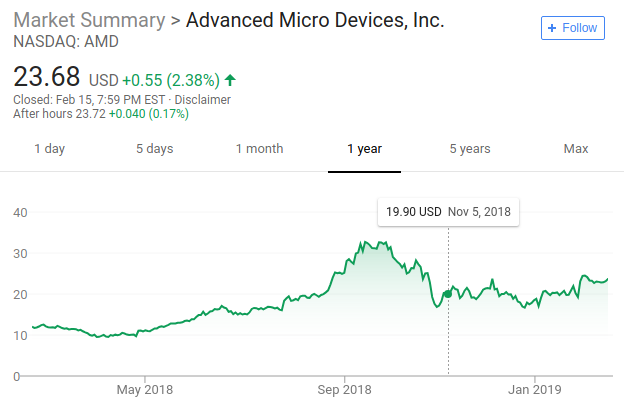
\includegraphics[width=\textwidth]{images/AMDChart.png}
			\caption{A chart of AMD stock prices}
			\label{AMD Chart}
		\end{subfigure}
		\begin{subfigure}[b]{.45\textwidth}
			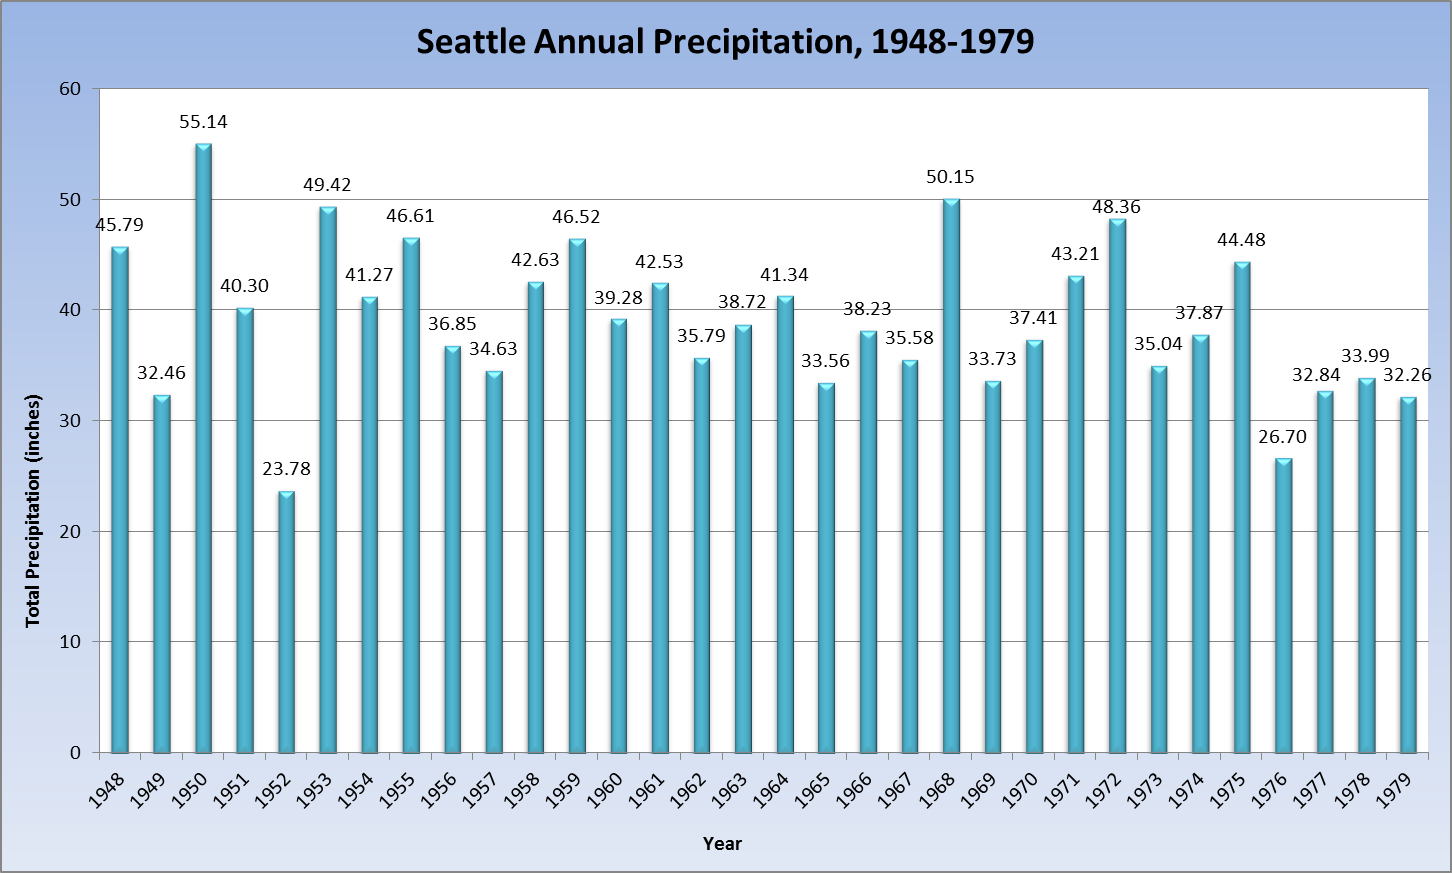
\includegraphics[width=\textwidth]{images/SeattleRainfall.png}
			\caption{Seattle precipitation, 1948-1979}
			\label{AMD Chart}
		\end{subfigure}
		\caption[Examples of Time Series]{Examples of Time Series \footnotemark}
		\label{TimeSeriesExamples}
			
	\end{figure}
\footnotetext{Seattle precipitation image courtesy of \href{http://www.seattleweatherblog.com/rain-stats/}{Seattle Weather Blog}}
	
	\textcolor{red}{Talk about ARIMA models}
	
	\chapter{Hierarchical Temporal Memory}
	
	\section{The Neocortex}
	
	\textcolor{red}{Vernon Mountcastle}
	
	\textcolor{red}{Overview of the neocortex}
	
	\textcolor{red}{Cortical Columns and Pyramidal Neurons}
	
	\begin{figure}[h!]
		\centering
		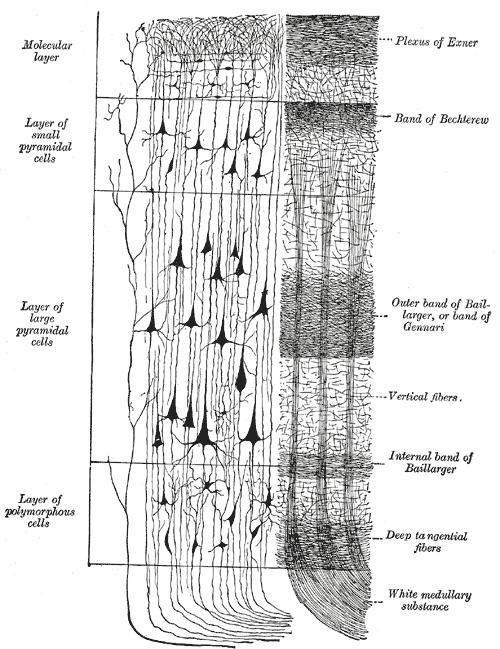
\includegraphics[width=8cm]{images/ColumnOfNeocortex.png}
		\caption{Column of the Neocortex}
		\label{CorticalColumn}
	\end{figure}
	
	\section{Sparse Distributed Representations}
	
	Consider the binary representation of the integer 16 versus that of the integer 15. The two numbers are quite similar: they are only 1 apart, so they are as close as two integers can be. Yet their binary representations are [100000] and [011111] respectively. They have no shared ``on'' bits so despite their similarity, their binary representations reflect none at all. In fact, despite being as close as two integers can be (a Euclidean distance of 1), their binary representations have a Hamming distance, the number places in which two codewords differ, of 5, the maximum Hamming distance of two codewords of length 5 \cite{Adams}. 
	
	This means that our encoding does not preserve semantic similarity or a concept of distance between elements which is highly undesirable for an code because if there is some kind of error in the code we could end up decoding something meaning the opposite of what we were trying to convey. As an example, consider $\mathbb{Z}$ from 0 to 31 which is mapped to $GF(2)^{6}$ by their binary representation. The mapping of 31 is [111111] but a single error in transmission can easily lead to [011111] which would be decoded as 15. So a code Hamming distance ($d_{H}$) of one away ($\frac{1}{5}$ of the total metric) lead to an element 16 integers away ($\frac{1}{2}$ of the total metric). We would obviously like to avoid this so that errors in the transmission of our codes are either (1) correctable or (2) lead to a decoding that is as close as possible to our original element.
	
	This is achievable by simply conveying more information in our code. In our binary representation any single error led to another valid codeword (a codeword which decoded to an element of the input/output set) which meant that no errors could be detected or corrected. By expanding our code length, we increase the number of codewords (multiplying by the cardinality of the code alphabet for each character added) meaning that fewer errors will result in other valid codewords and can possibly be detected or corrected. 
	
	A key strategy with Sparse Distributed Representations is to encode semantic similarity, such as with our idea of distance in our motivating example. This helps us achieve our second goal because even if we increase the error-tolerance of our code, there is still some probability of an uncorrectable error and we would like that error to result in a codeword as close to the original codeword as possible. To give you a real world example imagine I am sending instructions to a aircraft and I need to tell it to turn down 7\textdegree~to start its descent. Obviously, an error resulting in 8\textdegree~or 6\textdegree~being interpretted by the pilot are both preferable to 90\textdegree.
	
	To achieve our goal, we employ sparse distributed representations or SDRs. Just as with traditional dense binary representations, we will represent sparse distributed representations as vectors over their code alphabet, in this case GF(2). We call them \textbf{sparse} distributed representations because these vectors typically only have a small proportion of the components as 1. We will use Numenta's notation of letting $w_{\overrightarrow{x}}$ denote the number of components in an SDR $\overrightarrow{x}$ that are 1, so $w_{\overrightarrow{x}} = \norm{x}_{1}$ \cite{Properties}.
	
	Given our definition of distance, we could say that two decodings of sparse distributed representations, $a$ and $b$, are equal if and only if the $d_{H}(a,b) = w_{a} = w_{b}$. This would mean that both vectors would have to have the same dimensionality, same number of on bits, and all on and off bits would have to match. This definition is good for ``equals,'' but suppose we have a single error in transmission or a single component of our distributed system fails, equality would thus fail. In order to be able preserve the ability to subsample and thus to preserve fault tolerance, we therefore need a less stringent definition for decoding SDRs. Numenta refers to this as the $overlap$, which is $$ overlap(\overrightarrow{a}, \overrightarrow{b}) \equiv \overrightarrow{a} \cdot \overrightarrow{b} \equiv \sum_{0}^{n-1} a_{i}b_{i}$$ Thus, we say two SDRs $\overrightarrow{a}$ and $\overrightarrow{b}$ decode to the same element of the input space if and only if $overlap(a,b) \geq \theta$ where $\theta \leq w_{a}$ and $\theta \leq w_{b}$ \cite{Properties}. Denote the function that determines if two sparse distributed representations decode to the same element of the input space using some $\theta$ and $overlap(\overrightarrow{a}, \overrightarrow{b})$, $match_{\theta}(\overrightarrow{a}, \overrightarrow{b})$ and it is a function from SDR$\times$SDR $\longrightarrow$\{true, false\}.
	
	Given a set of sparse distributed representations with the same dimension, $X =\{\overrightarrow{x_{1}}, \overrightarrow{x_{2}}, ...,\overrightarrow{x_{n}}\}$, we can union the vectors using the bitwise OR operation over the $i^{th}$ position of the vectors in the set to produce the $i^{th}$ position of $union(X)$ \cite{Properties}. For example, given [0100] and [0010] the union would be [0110]. We say an SDR $\overrightarrow{y}$ is an element of the union of a set of SDRs, $\overrightarrow{X}$, if and only if $match_{\theta}(\overrightarrow{X},\ \overrightarrow{y})$ \cite{Properties}.
	
	\section{Cortical Learning Algorithms}
	
	\textcolor{red}{Sequence memory - SDRs and transitions}
	
	\textcolor{red}{Variable order sequence memory - cells per minicolumn}
	
	
	\begin{figure}[h!]
		\centering
		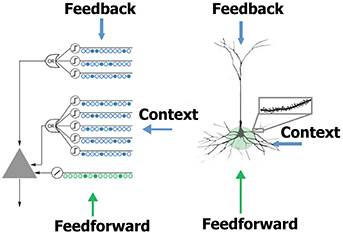
\includegraphics[width=\linewidth]{images/HTMCell.jpg}
		\caption{Hierarchical Temporal Memory Cell}
		\label{fig 1}
	\end{figure}

	\begin{figure}[h!]
		\centering
		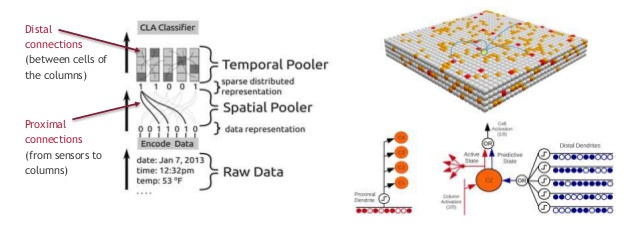
\includegraphics[width=\linewidth]{images/Poolers.jpg}
		\caption{Spatial and Temporal Poolers}
		\label{fig 2}
	\end{figure}

	\subsection{Classifier}
	
	Once the system completes its processing of a time step's input, the system outputs a sparse distributed representation which may have gone through multiple layers and it is important to be able to decode the system's prediction in order for the system to be useful. Hierarchical Temporal Memory currently uses something called an SDR Classifier to decode the predictions of an HTM \cite{Dillon}. At its essence, an SDR Classifier is a single layer, feed forward, neural network \cite{Dillon}.
	
	\begin{figure}[h!]
		\centering
		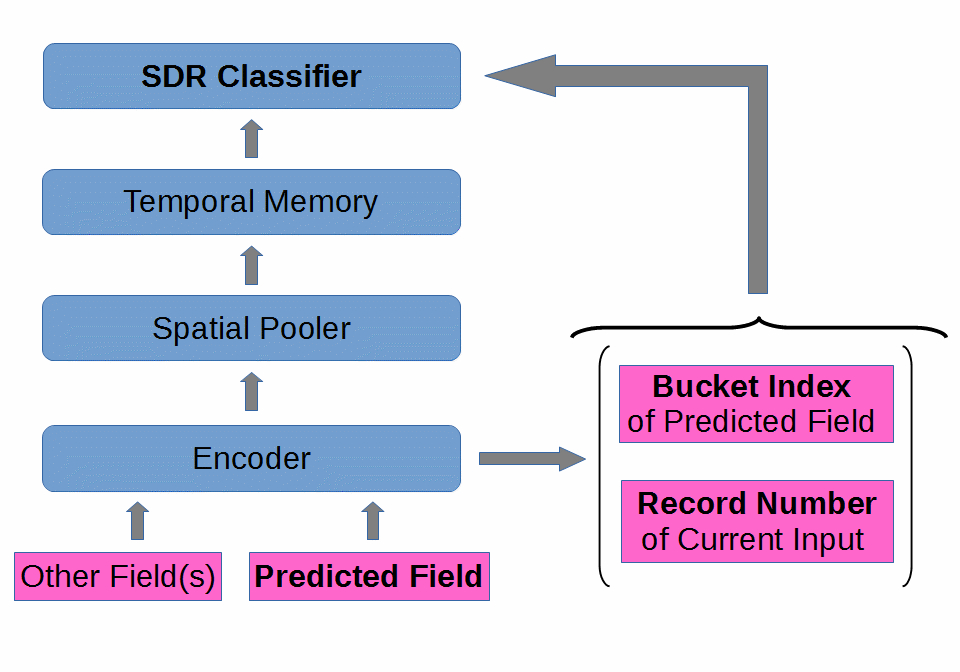
\includegraphics[width=\linewidth]{images/SDRClassifier.jpg}
		\caption{SDR Classifier}
		\label{fig 3}
	\end{figure}
	
	SDR Classifiers are able to decode the information HTMs give about predictions $n$ times steps in the future by maintaining a weight matrix \cite{Dillon}. The matrix's weights are adjusted to ``learn'' after each time step to reflect the correct weighting between the output vector at time $t$ and the probability distribution of the input/output space at time $t-n$ \cite{Dillon}. This enables the matrix to reflect relationships between inputs and outputs $n$ time steps apart. To determine the SDR Classifier's interpretation of an output at time $t+n$, the SDR Classifer takes in the HTM's output vector and uses Softmax to determine the most likely decoding \cite{Dillon}. So for each of the $k$ classes in the output space, the certainty that the output vector is referring to it is $$y_{j} = \dfrac{e^{a_{j}}}{\sum_{i=1}^{k} e^{a_{i}}}$$ where $a_{j}$ is the activation level of the $j^{th}$ element of the output space, calculated by multiplying the output vector by the $j^{th}$ column of the weight matrix element wise \cite{Dillon}. 
	
	\chapter{Literature Review}
	
	\textcolor{red}{Does anyone know if its able to do this?}
	
	\textcolor{red}{It has been used in applications, look there}
	
	\textcolor{red}{partners such as http://numenta.com/htm-for-stocks/ grokstream.com cortical.io}
	
	\chapter{Experiment Design}
	
	\section{Hardware and Software Specifications}
	
	I utilized the official Python (Python 2.7) implementation of Numenta's cortical learning algorithms, NuPIC\footnote{NuPIC repository: \href{https://github.com/numenta/nupic}{\ttfamily https://github.com/numenta/nupic} } and it's Network API\footnote{Network API docs: \href{http://nupic.docs.numenta.org/stable/api/network/}{\ttfamily http://nupic.docs.numenta.org/stable/api/network/}}. At the time of my work NuPIC was at version 1.05 and I chose to use this version. It should be noted that although much of NuPIC is in Python, many of its computationally intensive algorithms are implemented in C++ using their NuPIC.core repository\footnote{NuPIC.core repository: \href{https://github.com/numenta/nupic.core}{\ttfamily https://github.com/numenta/nupic.core}} and it also relies on a number of external libraries such as \texttt{numpy} and \texttt{pandas}. 
	
	Due to the computationally intensive nature of my research and the limited time available to me, I also heavily relied on parallel processing to run my code in a reasonable time frame. In particular, the \texttt{multiprocessing} package in Python was indispensable to my research, allowing me to speed my code up a factor of up to 20$\times$ when running independent tests or swarming.
	
	\begin{table}[h!]
		\centering
		\begin{tabular}{|l|l|}
			\hline
			\multicolumn{2}{|l|}{Dijkstra (Asus Vivobook)} \\ \hline
			CPU     & Intel i5-8250U, 4-Core, 1.60GHz     \\ \hline
			RAM     & 24 GB                                \\ \hline
			OS      & Linux Mint 19 Cinnamon               \\ \hline
			\multicolumn{2}{|l|}{Galois (HP DL380 G7)}     \\ \hline
			CPU     &  Intel Xeon X5650, 6-Core, 2.70 GHz       \\ \hline
			RAM     & 192 GB                               \\ \hline
			OS      & Linux Mint 19 Cinnamon               \\ \hline
			\multicolumn{2}{|l|}{}                         \\ \hline
			&                                      \\ \hline
			&                                      \\ \hline
			&                                      \\ \hline
		\end{tabular}
		\caption{Hardware Specifications}
		\label{tab:hardware}
	\end{table}

	On the hardware side of things, the majority of development and testing was conducted on my personal laptop, an Asus Vivobook with some small upgrades (see Table~\ref{tab:hardware} for details). The code was then deployed to my HP DL380 G7 server which had more cores, more memory, and a higher clock speed allowing me to get faster results. For a synopsis of the hardware specifications, see Table~\ref{tab:hardware}. 
	
	\textcolor{red}{Hardware and language}
	
	\textcolor{red}{Numerical analysis-Epsilon comparisons}
	
	\section{Particle Swarm Optimization}
	
	Introduced in by Russell Eberhart and James Kennedy in their 1995 paper, \textit{A New Optimizer Using Particle Swarm Theory}, Particle Swarm Optimization has changed the way the world optimizes continuous nonlinear functions. Usually abbreviated to PSO or \textit{swarming}, it draws inspiration from bird flocks and schools of fish \cite{Eberhart}. The concept is quite simple: it simulates particles on parameter space and at each time-step each particle evaluates fitness as a function of its location in parameter space, then moves towards some linear combination of its personal best and the overall best score among the particles.
	
	\textcolor{red}{Wrote wrapper and swarming utility}
	
	\textcolor{red}{LOTS of swarming}
	
	\chapter{Results and Discussion}
	
	\chapter{Further Work}
	
	
	
	\blankpage
	\addcontentsline{toc}{chapter}{References}
	\bibliographystyle{siam}     % Siam and Ieeetr bibliographic styles treat titles of articles in journals or collections correctly
	\nocite{*}  % List ALL references in your references, not just the ones cited in the text.
	% This scheme automatically alphabetizes the Bibliography.
	\bibliography{Bibliography}{}
	
	\appendices
	\addcontentsline{toc}{chapter}{Appendix}
	
\end{document}
